
\section{Goal of the project}
\begin{frame}

%\frametitle{Goal of the project}



%Columns which are aligned with the first ligne for basis
\begin{columns}[t]

%%%%%%%%%%%%%%%%%%%%%%%%%%%%%%%%%%%%%%%%%%%%%%%%%%
%	CRYPTO WRAP									 %
%%%%%%%%%%%%%%%%%%%%%%%%%%%%%%%%%%%%%%%%%%%%%%%%%%
\begin{column}{0.375\textwidth}

%%---------------------------------------------------------------------------------------------------
% Settings
%---------------------------------------------------------------------------------------------------
\newcommand{\mypapersize}{A4}
\newcommand{\mylaterality}{oneside}
%% "oneside" or "twoside"
\newcommand{\mydraft}{false}
%% "true" or "false"
\newcommand{\myparskip}{half}
%% e.g., "no", "full", "half", ...
\newcommand{\myBCOR}{10mm}
\newcommand{\myfontsize}{11pt}   
\newcommand{\mylinespread}{onehalfspacing} 
%% e.g.onehalfspacing, doublespacing, singlespacing
%% Line spacing in %/100. For example 1.5 means 150% of the usual line
%% spacing. Please use with caution: 100% ("1.0") is fine because the
%% font was designed for it.
\newcommand{\mylanguage}{ngerman,american}
%% NOTE: The *last* language is the active one!
%% BibLaTeX-settings: (see biblatex reference for further description)
\newcommand{\mybiblatexstyle}{numeric}
%% e.g., "alphabetic", "authoryear", ...
%% The biblatex style which is being used for referencing. See
%% biblatex documentation for further details and more values.
%%
%% CAUTION: if you change the style, please check for (in)compatible
%%          "biblatex" package options in the file
%%          "template/preamble.tex"! For example: "alphabetic" does
%%          not have an option "dashed=..." and causes an error if it
%%          does not get removed from the list of options.

\newcommand{\mybiblatexdashed}{false}  %% "true" or "false"
%% If true: replace recurring reference authors with a dash.

\newcommand{\mybiblatexbackref}{true}  %% "true" or "false"
%% If true: create backward links from reference to citations.

\newcommand{\mybiblatexfile}{bib/bibliography.bib}
%% Name of the biblatex file that holds the references.

\newcommand{\mydispositioncolor}{0,0,0}
%% e.g., "30,103,182" (blue/turquois), "0,0,0" (black), ...
%% Color of the headings and so forth in RGB (red,green,blue) values.

\newcommand{\mycolorlinks}{false}  %% "true" or "false"
%% Enables or disables colored links (hyperref package).
\newcommand{\mytodonotesoptions}{disable}
%% e.g., "" (empty), "disable", ...
%% Options for the todonotes-package. If "disable", all todonotes will
%% be hidden (including todos).
%% ========================================================================
%%  Document metadata
%% ========================================================================
%% general metadata:
\newcommand{\myauthor}{Steve Wagner}  %% also used for PDF metadata
% (hyperref)
\newcommand{\myformation}{EI-3nat}
\newcommand{\mytitle}{Bachelor Thesis}  %% also used for PDF metadata (hyperref)
\newcommand{\mysubject}{Extension and Integration of an Abstract Interface to Cryptography Providers}  %% also used for PDF metadata (hyperref)
\newcommand{\mykeywords}{<++keywords++>}  %% also used for PDF metadata (hyperref)
%% this information is used only for generating the title page:
\newcommand{\myworktitle}{Bachelor thesis}  %% official type of work like ``Master theses''
\newcommand{\mygrade}{Bachelor of Engineering} %% title you are getting with this work like ``Master of ...''
\newcommand{\mystudy}{Electronik und Informationstechnik} %% your study like ``Arts''
\newcommand{\myuniversity}{Offenburg University of Applied Sciences} %% your
% university/school
\newcommand{\myinstitute}{Institute of reliable Embedded Systems and
Communication Electronics (ivESK)}
%% affiliation
\newcommand{\myinstitutehead}{Prof. Dr. Axel Sikora} %% head of institute 
\newcommand{\mysupervisor}{Dipl.-Phys. Andreas Walz} %% your supervisor
\newcommand{\myevaluator}{myprof} %% your evaluator
\newcommand{\myhomestreet}{street} %% your home street (with house number)
\newcommand{\myhometown}{town} %% your home town
\newcommand{\myhomepostalnumber}{psn} %% your postal number of home town
\newcommand{\mysubmissionmonth}{month} %% month you are handing in
\newcommand{\mysubmissionyear}{year} %% year you are handing in
\newcommand{\mysubmissiontown}{\myhometown} %% town of handing in (or \myhometown)
%% additional information for generic_documentation title page

%---------------------------------------------------------------------------------------------------
% formating
%---------------------------------------------------------------------------------------------------

\newcommand{\clearemptydoublepage}{\clearpage\newpage\thispagestyle{empty}\cleardoublepage}

\newcommand{\CRule}{\rule{0.95\textwidth}{0.5pt}} % New command to make the lines above figure captions


%---------------------------------------------------------------------------------------------------
% fixme makro
%---------------------------------------------------------------------------------------------------

%\newcommand{\fixme}[1]{\textbf{\large FIXME: #1}}
%\newcommand{\todo}[1]{\textbf{\large TODO: #1}}
%\newcommand{\idea}[1]{\textbf{IDEA: #1 ~\\}}


%---------------------------------------------------------------------------------------------------
% names
%---------------------------------------------------------------------------------------------------

\newcommand{\gci}{Generic Cryptographic Interface (GCI)\xspace}
\newcommand{\embtls}{emb::TLS\xspace}
\newcommand{\tomcrypt}{LibTomCrypt\xspace}
\newcommand{\vaultic}{VaultIC\num{460}\xspace}
\newcommand{\Table}{Table}
\newcommand{\Tables}{Tables}
\newcommand{\Figure}{Figure}
\newcommand{\Figures}{Figures}
\newcommand{\Subfigure}{Subfigure}
\newcommand{\Section}{Section}
\newcommand{\Sections}{Sections}
\newcommand{\Chapter}{Chapter}
\newcommand{\Chapters}{Chapters}
\newcommand{\Equation}{Equation}
\newcommand{\Equations}{Equations}

\newcommand{\Appendix}{Appendix}
\newcommand{\Appendices}{Appendices}
\newcommand{\Ref}{Ref.}
\newcommand{\Refs}{Refs.}

%---------------------------------------------------------------------------------------------------
% units
%---------------------------------------------------------------------------------------------------

\newcommand{\Hz}	{\ensuremath{\mathrm{Hz}}\xspace}
\newcommand{\kHz}	{\ensuremath{\mathrm{kHz}}\xspace}
\newcommand{\MHz}	{\ensuremath{\mathrm{MHz}}\xspace}

\newcommand{\cm}{\ensuremath{\mathrm{cm}}\xspace}
\newcommand{\m}{\ensuremath{\mathrm{m}}\xspace}
\newcommand{\mm}{\ensuremath{\mathrm{mm}}\xspace}
\newcommand{\microm}{\ensuremath{\mu\mathrm{m}}\xspace}
\newcommand{\s}{\ensuremath{\mathrm{s}}\xspace}
\newcommand{\musec}{\ensuremath{\mu\mathrm{s}}\xspace}


%---------------------------------------------------------------------------------------------------
% include figures
%---------------------------------------------------------------------------------------------------
\newcommand{\myfig}[5]{
%% example:
% \myfig{}%% filename in figures folder
%       {width=0.5\textwidth,height=0.5\textheight}%% maximum width/height, aspect ratio will be kept
%       {}%% caption
%       {}%% optional (short) caption for list of figures
%       {}%% label
\begin{figure}%[htp]
  \begin{center}
     \includegraphics[keepaspectratio,#2]{figures/#1}
     \caption[#4]{#3}
     \label{#5} %% NOTE: always label *after* caption!
  \end{center}
  
\end{figure}
}




\documentclass{beamer}


%%=====================================================================================
%% drawing tikz
%%=====================================================================================
%
\usepackage{tikz}
\usetikzlibrary{positioning,shapes,arrows}%
\tikzstyle{memblock} = [draw, fill=blue!20, rectangle, 
    minimum height=6em, minimum width=3em]%
\definecolor{mygray}{cmyk}{0,0,0,0.4}%
\definecolor{mydarkgray}{cmyk}{0,0,0,0.7}%
\definecolor{mylightgray}{cmyk}{0,0,0,0.1}%

%________________________________________________________________
%tikz flow chart
\tikzstyle{decision} = [diamond, draw, fill=blue!20, 
    text width=4.25em, text badly centered, node distance=2cm, inner sep=0pt]
\tikzstyle{block} = [rectangle, draw, fill=blue!20, 
     text centered, rounded corners, minimum height=1.5em] 
     
\tikzstyle{block2} = [rectangle, draw, fill=orange!20, 
     text centered, rounded corners, minimum height=1.5em] 
     
\tikzstyle{block3} = [rectangle, draw, fill=green!20, 
     text centered, rounded corners, minimum height=1.5em] 
     
\tikzstyle{rect} = [rectangle, draw, fill=blue!20, text centered, minimum
height=1.5em, minimum width=5em]
    
    
    
\tikzstyle{line} = [draw, -latex']
\tikzstyle{cloud} = [draw, ellipse,fill=red!20, node distance=2cm,
    minimum height=1em]
    
\tikzstyle{txtblk} = [above, text centered]

% Define the layers to draw the diagram
\pgfdeclarelayer{background}
\pgfdeclarelayer{foreground}
\pgfsetlayers{background,main,foreground}

\begin{document}

\begin{tikzpicture}[node distance=2.25cm]

%%%%%%%%%%%%%%%%%%%%%%%%%%%%%%%%%%%%%%%%%%%%%%%%%%
%	Application									 %
%%%%%%%%%%%%%%%%%%%%%%%%%%%%%%%%%%%%%%%%%%%%%%%%%%

% Create a node
\node (embtls) [block, text width=5.5em]{\embtls};

\path (embtls.north)+(0,0.85) node (txtcw) [txtblk] {\underline{\small{Use of
the old interface:}}};

% Create a text which in coordinate (-2,-0.5) of the middle of the south of
% embtls node
\path (embtls.south) +(-1.85,-0.4) node (app) [text width=0.5] {Application};


% This allow to create the rectangle
\begin{pgfonlayer}{background}
	  
  	%create  the lines of the rectangle  with an offset (x,y)         
	\path (embtls.west |- embtls.north)+(-0.75,0.65) node (a) {};
  	\path (embtls.south -|  embtls.east)+(0.75,-0.65) node (b) {};      
          
    % Combine the twos nodes above for creating the rectangle      
    \path[fill=mylightgray!20,rounded corners, draw=black!50, dashed]
    (a) rectangle (b);  
            
\end{pgfonlayer}

%%%%%%%%%%%%%%%%%%%%%%%%%%%%%%%%%%%%%%%%%%%%%%%%%%
%	Interface									 %
%%%%%%%%%%%%%%%%%%%%%%%%%%%%%%%%%%%%%%%%%%%%%%%%%%
\node (cryptw) [block, below of=embtls, text width=5.5em, fill=red!60]{Crypto
Wrap};

\path (cryptw.south) +(-1.85,-0.4) node (int1) [text width=0.5] {Interface};

\begin{pgfonlayer}{background}
          
   	\path (cryptw.west |- cryptw.north)+(-0.75,0.65) node (c) {};
   	\path (cryptw.south -|  cryptw.east)+(0.75,-0.65) node (d) {};
          
	\path[fill=mylightgray!20,rounded corners, draw=black!50, dashed]
    (c) rectangle (d);           
            
\end{pgfonlayer}


%%%%%%%%%%%%%%%%%%%%%%%%%%%%%%%%%%%%%%%%%%%%%%%%%%
%	Crypto provider								 %
%%%%%%%%%%%%%%%%%%%%%%%%%%%%%%%%%%%%%%%%%%%%%%%%%%
\node (tomcr) [block, below of=cryptw, text width=5.5em]{\tomcrypt};

\path (tomcr.south) +(-0.65,-0.4) node (lib){Crypto provider};

\begin{pgfonlayer}{background}
          
   \path (tomcr.west |- tomcr.north)+(-0.75,0.65) node (e) {};
   \path (tomcr.south -|  tomcr.east)+(0.75,-0.65) node (f) {};  
                   
   \path[fill=mylightgray!20,rounded corners, draw=black!50, dashed]
   (e) rectangle (f);           
            
\end{pgfonlayer}


\path [draw, ->] (tomcr.north) -- (cryptw.south);
\path [draw, ->] (cryptw.north) -- (embtls.south);


\end{tikzpicture}

\end{document}
% trim: left, bottom, right, up
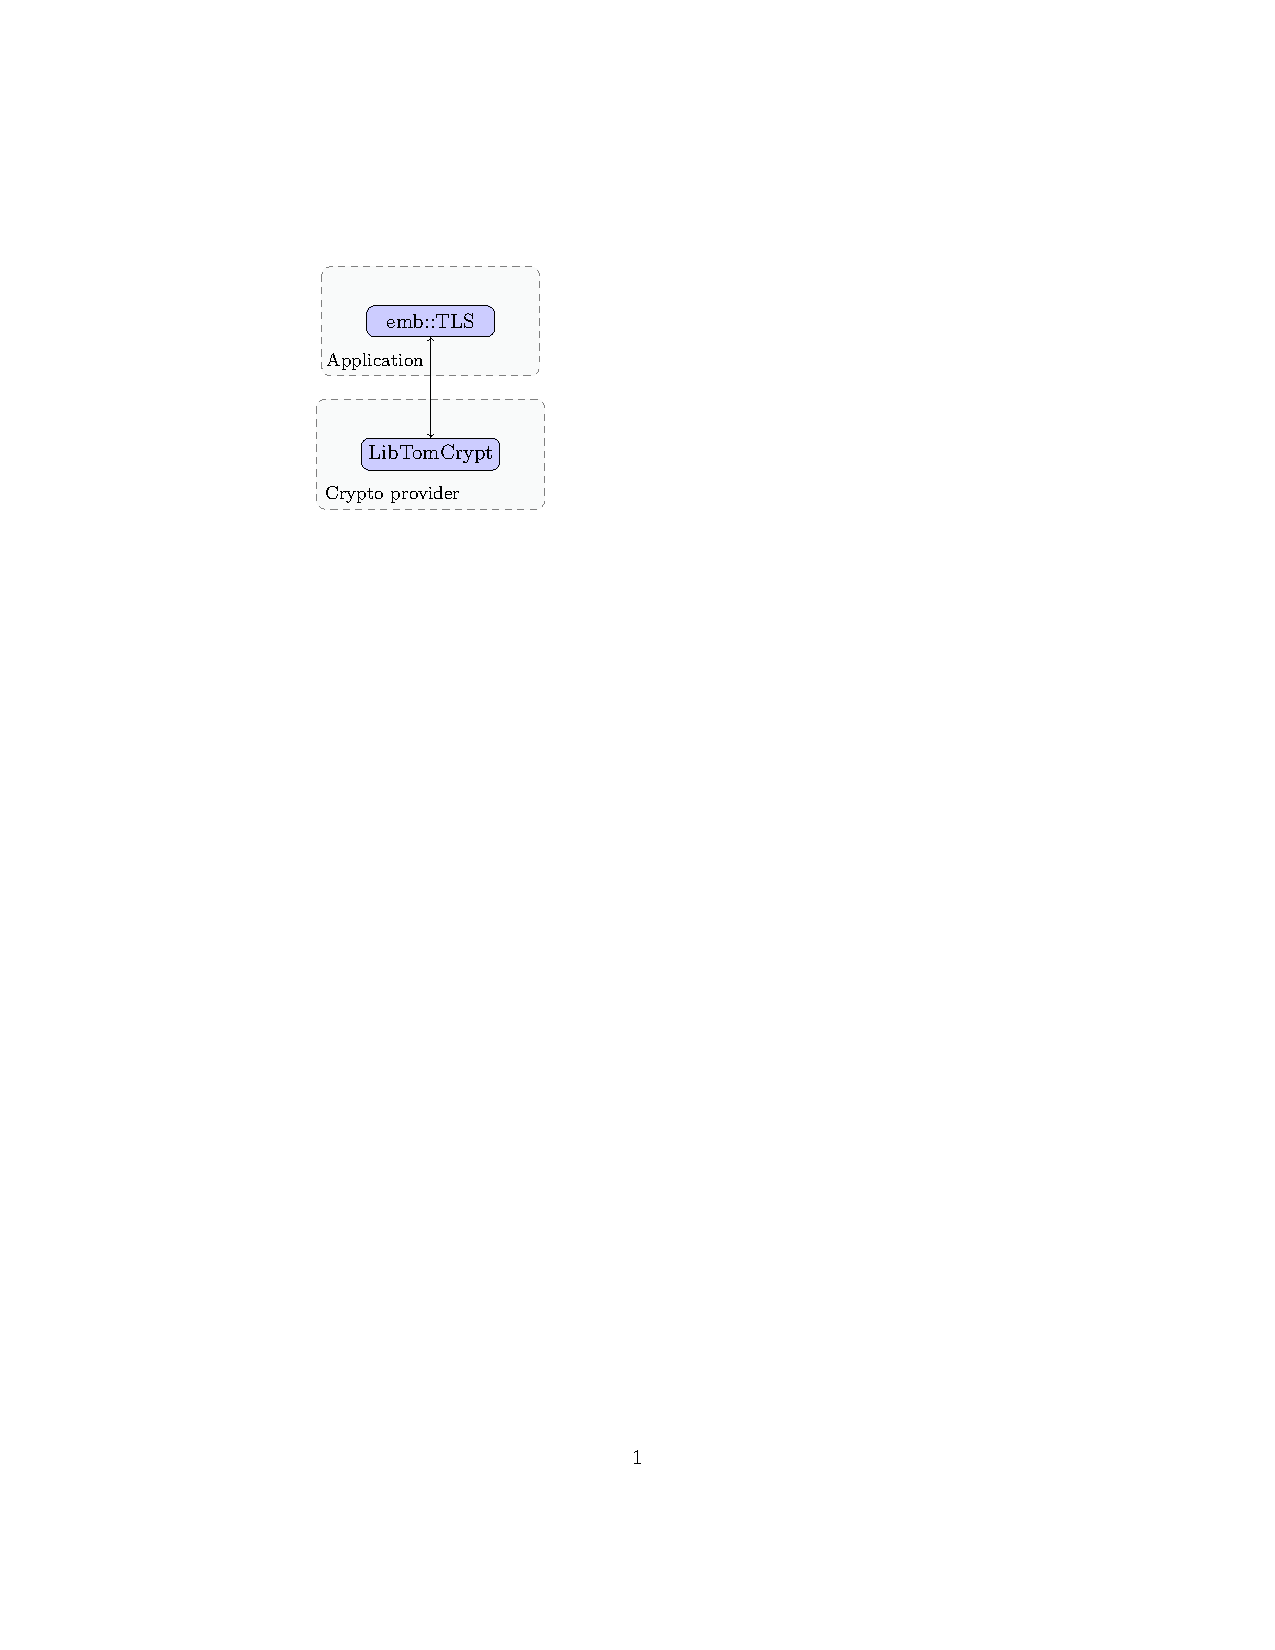
\includegraphics[trim=1cm 1cm 14cm 0cm, height=8cm]{figures/intro_cw.pdf}


\end{column}

%%%%%%%%%%%%%%%%%%%%%%%%%%%%%%%%%%%%%%%%%%%%%%%%%%
%	GCI											 %
%%%%%%%%%%%%%%%%%%%%%%%%%%%%%%%%%%%%%%%%%%%%%%%%%%
\begin{column}{0.725\textwidth}

%%---------------------------------------------------------------------------------------------------
% Settings
%---------------------------------------------------------------------------------------------------
\newcommand{\mypapersize}{A4}
\newcommand{\mylaterality}{oneside}
%% "oneside" or "twoside"
\newcommand{\mydraft}{false}
%% "true" or "false"
\newcommand{\myparskip}{half}
%% e.g., "no", "full", "half", ...
\newcommand{\myBCOR}{10mm}
\newcommand{\myfontsize}{11pt}   
\newcommand{\mylinespread}{onehalfspacing} 
%% e.g.onehalfspacing, doublespacing, singlespacing
%% Line spacing in %/100. For example 1.5 means 150% of the usual line
%% spacing. Please use with caution: 100% ("1.0") is fine because the
%% font was designed for it.
\newcommand{\mylanguage}{ngerman,american}
%% NOTE: The *last* language is the active one!
%% BibLaTeX-settings: (see biblatex reference for further description)
\newcommand{\mybiblatexstyle}{numeric}
%% e.g., "alphabetic", "authoryear", ...
%% The biblatex style which is being used for referencing. See
%% biblatex documentation for further details and more values.
%%
%% CAUTION: if you change the style, please check for (in)compatible
%%          "biblatex" package options in the file
%%          "template/preamble.tex"! For example: "alphabetic" does
%%          not have an option "dashed=..." and causes an error if it
%%          does not get removed from the list of options.

\newcommand{\mybiblatexdashed}{false}  %% "true" or "false"
%% If true: replace recurring reference authors with a dash.

\newcommand{\mybiblatexbackref}{true}  %% "true" or "false"
%% If true: create backward links from reference to citations.

\newcommand{\mybiblatexfile}{bib/bibliography.bib}
%% Name of the biblatex file that holds the references.

\newcommand{\mydispositioncolor}{0,0,0}
%% e.g., "30,103,182" (blue/turquois), "0,0,0" (black), ...
%% Color of the headings and so forth in RGB (red,green,blue) values.

\newcommand{\mycolorlinks}{false}  %% "true" or "false"
%% Enables or disables colored links (hyperref package).
\newcommand{\mytodonotesoptions}{disable}
%% e.g., "" (empty), "disable", ...
%% Options for the todonotes-package. If "disable", all todonotes will
%% be hidden (including todos).
%% ========================================================================
%%  Document metadata
%% ========================================================================
%% general metadata:
\newcommand{\myauthor}{Steve Wagner}  %% also used for PDF metadata
% (hyperref)
\newcommand{\myformation}{EI-3nat}
\newcommand{\mytitle}{Bachelor Thesis}  %% also used for PDF metadata (hyperref)
\newcommand{\mysubject}{Extension and Integration of an Abstract Interface to Cryptography Providers}  %% also used for PDF metadata (hyperref)
\newcommand{\mykeywords}{<++keywords++>}  %% also used for PDF metadata (hyperref)
%% this information is used only for generating the title page:
\newcommand{\myworktitle}{Bachelor thesis}  %% official type of work like ``Master theses''
\newcommand{\mygrade}{Bachelor of Engineering} %% title you are getting with this work like ``Master of ...''
\newcommand{\mystudy}{Electronik und Informationstechnik} %% your study like ``Arts''
\newcommand{\myuniversity}{Offenburg University of Applied Sciences} %% your
% university/school
\newcommand{\myinstitute}{Institute of reliable Embedded Systems and
Communication Electronics (ivESK)}
%% affiliation
\newcommand{\myinstitutehead}{Prof. Dr. Axel Sikora} %% head of institute 
\newcommand{\mysupervisor}{Dipl.-Phys. Andreas Walz} %% your supervisor
\newcommand{\myevaluator}{myprof} %% your evaluator
\newcommand{\myhomestreet}{street} %% your home street (with house number)
\newcommand{\myhometown}{town} %% your home town
\newcommand{\myhomepostalnumber}{psn} %% your postal number of home town
\newcommand{\mysubmissionmonth}{month} %% month you are handing in
\newcommand{\mysubmissionyear}{year} %% year you are handing in
\newcommand{\mysubmissiontown}{\myhometown} %% town of handing in (or \myhometown)
%% additional information for generic_documentation title page

%---------------------------------------------------------------------------------------------------
% formating
%---------------------------------------------------------------------------------------------------

\newcommand{\clearemptydoublepage}{\clearpage\newpage\thispagestyle{empty}\cleardoublepage}

\newcommand{\CRule}{\rule{0.95\textwidth}{0.5pt}} % New command to make the lines above figure captions


%---------------------------------------------------------------------------------------------------
% fixme makro
%---------------------------------------------------------------------------------------------------

%\newcommand{\fixme}[1]{\textbf{\large FIXME: #1}}
%\newcommand{\todo}[1]{\textbf{\large TODO: #1}}
%\newcommand{\idea}[1]{\textbf{IDEA: #1 ~\\}}


%---------------------------------------------------------------------------------------------------
% names
%---------------------------------------------------------------------------------------------------

\newcommand{\gci}{Generic Cryptographic Interface (GCI)\xspace}
\newcommand{\embtls}{emb::TLS\xspace}
\newcommand{\tomcrypt}{LibTomCrypt\xspace}
\newcommand{\vaultic}{VaultIC\num{460}\xspace}
\newcommand{\Table}{Table}
\newcommand{\Tables}{Tables}
\newcommand{\Figure}{Figure}
\newcommand{\Figures}{Figures}
\newcommand{\Subfigure}{Subfigure}
\newcommand{\Section}{Section}
\newcommand{\Sections}{Sections}
\newcommand{\Chapter}{Chapter}
\newcommand{\Chapters}{Chapters}
\newcommand{\Equation}{Equation}
\newcommand{\Equations}{Equations}

\newcommand{\Appendix}{Appendix}
\newcommand{\Appendices}{Appendices}
\newcommand{\Ref}{Ref.}
\newcommand{\Refs}{Refs.}

%---------------------------------------------------------------------------------------------------
% units
%---------------------------------------------------------------------------------------------------

\newcommand{\Hz}	{\ensuremath{\mathrm{Hz}}\xspace}
\newcommand{\kHz}	{\ensuremath{\mathrm{kHz}}\xspace}
\newcommand{\MHz}	{\ensuremath{\mathrm{MHz}}\xspace}

\newcommand{\cm}{\ensuremath{\mathrm{cm}}\xspace}
\newcommand{\m}{\ensuremath{\mathrm{m}}\xspace}
\newcommand{\mm}{\ensuremath{\mathrm{mm}}\xspace}
\newcommand{\microm}{\ensuremath{\mu\mathrm{m}}\xspace}
\newcommand{\s}{\ensuremath{\mathrm{s}}\xspace}
\newcommand{\musec}{\ensuremath{\mu\mathrm{s}}\xspace}


%---------------------------------------------------------------------------------------------------
% include figures
%---------------------------------------------------------------------------------------------------
\newcommand{\myfig}[5]{
%% example:
% \myfig{}%% filename in figures folder
%       {width=0.5\textwidth,height=0.5\textheight}%% maximum width/height, aspect ratio will be kept
%       {}%% caption
%       {}%% optional (short) caption for list of figures
%       {}%% label
\begin{figure}%[htp]
  \begin{center}
     \includegraphics[keepaspectratio,#2]{figures/#1}
     \caption[#4]{#3}
     \label{#5} %% NOTE: always label *after* caption!
  \end{center}
  
\end{figure}
}




\documentclass{article}


%%=====================================================================================
%% drawing tikz
%%=====================================================================================
%
\usepackage{tikz}
\usetikzlibrary{positioning,shapes,arrows}%
\tikzstyle{memblock} = [draw, fill=blue!20, rectangle, 
    minimum height=6em, minimum width=3em]%
\definecolor{mygray}{cmyk}{0,0,0,0.4}%
\definecolor{mydarkgray}{cmyk}{0,0,0,0.7}%
\definecolor{mylightgray}{cmyk}{0,0,0,0.1}%

\usepackage[margin=0.5cm]{geometry}

%________________________________________________________________
%tikz flow chart
\tikzstyle{decision} = [diamond, draw, fill=blue!20, 
    text width=4.25em, text badly centered, node distance=2cm, inner sep=0pt]
\tikzstyle{block} = [rectangle, draw, fill=blue!20, 
     text centered, rounded corners, minimum height=1.5em] 
     
\tikzstyle{block2} = [rectangle, draw, fill=orange!20, 
     text centered, rounded corners, minimum height=1.5em] 
     
\tikzstyle{block3} = [rectangle, draw, fill=green!20, 
     text centered, rounded corners, minimum height=1.5em] 
     
\tikzstyle{rect} = [rectangle, draw, fill=blue!20, text centered, minimum
height=1.5em, minimum width=5em]
    
    
    
\tikzstyle{line} = [draw, -latex']
\tikzstyle{cloud} = [draw, ellipse,fill=red!20, node distance=2cm,
    minimum height=1em]
    
\tikzstyle{txtblk} = [above, text centered]

% Define the layers to draw the diagram
\pgfdeclarelayer{background}
\pgfdeclarelayer{foreground}
\pgfsetlayers{background,main,foreground}

\begin{document}


\begin{tikzpicture}[node distance=2.25cm]



%%%%%%%%%%%%%%%%%%%%%%%%%%%%%%%%%%%%%%%%%%%%%%%%%%
%	Application									 %
%%%%%%%%%%%%%%%%%%%%%%%%%%%%%%%%%%%%%%%%%%%%%%%%%%

% Create a node
\node (embtls) [block, text width=5.5em]{\embtls};

\path (embtls.east)+(-3.25,0) node (other1) [block, text width=2.5em] {\ldots};
\path (embtls.west)+(3.25,0) node (other2) [block, text width=2.5em] {\ldots};

% Create a text which in coordinate (-2,-0.5) of the middle of the south of
% embtls node
\path (embtls.south) +(-4,-0.4) node (app) [text width=0.5] {Applications};

% This allow to create the rectangle
\begin{pgfonlayer}{background}
	  
  	%create  the lines of the rectangle  with an offset (x,y)         
	\path (other1.west |- other1.north)+(-1.75,0.65) node (a) {};
  	\path (other2.south -|  other2.east)+(0.5,-0.65) node (b) {};      
          
    % Combine the twos nodes above for creating the rectangle      
    \path[fill=mylightgray!20,rounded corners, draw=black!50, dashed]
    (a) rectangle (b);  
             
    \path (embtls.north west)+(-0.2,0.2) node (blank) {};
            
\end{pgfonlayer}

%%%%%%%%%%%%%%%%%%%%%%%%%%%%%%%%%%%%%%%%%%%%%%%%%%
%	Interface									 %
%%%%%%%%%%%%%%%%%%%%%%%%%%%%%%%%%%%%%%%%%%%%%%%%%%

\node (cryptw) [block, below of=embtls, text width=5.5em, fill=green!60]{GCI};

\path (cryptw.south) +(-4,-0.4) node (int1) [text width=0.5] {Interface};

\begin{pgfonlayer}{background}
          
   	\path (cryptw.west |- cryptw.north)+(-3.25,0.65) node (c) {};
   	\path (cryptw.south -|  cryptw.east)+(2,-0.65) node (d) {};
          
	\path[fill=mylightgray!20,rounded corners, draw=black!50, dashed]
    (c) rectangle (d);           
            
\end{pgfonlayer}


%%%%%%%%%%%%%%%%%%%%%%%%%%%%%%%%%%%%%%%%%%%%%%%%%%
%	Crypto provider								 %
%%%%%%%%%%%%%%%%%%%%%%%%%%%%%%%%%%%%%%%%%%%%%%%%%%
\node (tomcr) [block, below of=cryptw]{\tomcrypt};
\path (tomcr.west)+(-1.5,0) node (vltc) [block, text width=5.5em] {\vaultic};
\path (tomcr.east)+(0.9,0) node (other) [block, text width=2.5em] {\ldots};

\path (tomcr.south) +(-2.75,-0.4) node (lib) {Crypto providers};

\begin{pgfonlayer}{background}
          
   \path (vltc.west |- tomcr.north)+(-0.5,0.65) node (e) {};
   \path (vltc.south -|  other.east)+(0.5,-0.65) node (f) {};  
                   
   \path[fill=mylightgray!20,rounded corners, draw=black!50, dashed]
   (e) rectangle (f);
            
\end{pgfonlayer}


\path [draw, ->] (tomcr.north) -- (cryptw.south);
\path [draw, ->] (vltc.north) -- (cryptw.210);
\path [draw, ->] (other.north) -- (cryptw.330);

\path [draw, ->] (cryptw.north) -- (embtls.south);
\path [draw, ->] (cryptw.north) -- (other1.south);
\path [draw, ->] (cryptw.north) -- (other2.south);


\end{tikzpicture}

\end{document}
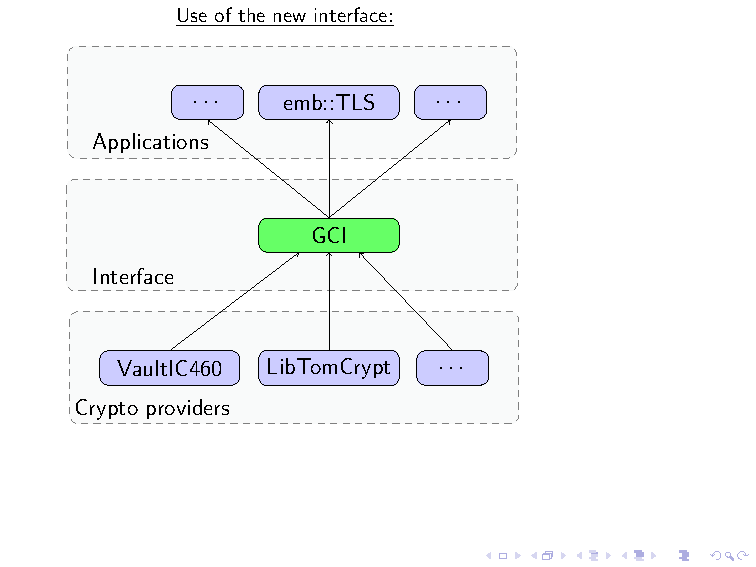
\includegraphics[trim=0.5cm 1cm 14cm 0cm, height=8cm]{figures/intro_gci.pdf}

\end{column}

\end{columns}

\end{frame}

\begin{frame}

\frametitle{Requirements}

\underline{Old cryptographic interface}:
\begin{itemize}

	\item Cannot be use in other application without changing some functions
	\item No other library can be use without rewriting the interface
	\item To old regarding the evolution of the cryptograhy

\end{itemize}

\vspace{0.5cm}

\underline{New cryptographc interface GCI}:
\begin{itemize}
  \item Possibility to use other cryptographic libraries
  \item Possibility to use it in hardware-coded-based cryptographic  
  modules
  \item Possibility to easily add new cryptographic algorithms

\end{itemize}

\end{frame}

\begin{frame}

\frametitle{Scheduling of the project}

\begin{enumerate}
  \item Acquisition of the basic cryptographic algorithms
  \vspace{0.25cm}
  \item Acquisition of TLS's princip and the implementation \embtls
  \vspace{0.25cm}
  \item Understanding the design of old cryptographic interface (Crypto Wrap)
  \vspace{0.25cm}
  \item Analysis of the cryptographic requirements imposed by TLS
  \vspace{0.25cm}
  \item Integration of the new interface in the application \embtls
  \vspace{0.25cm}
  \item Implementation of the provider \tomcrypt 
\end{enumerate}





\end{frame}




